%%%%%%%%%%%%%%%%%%%%%%%%%%%%%%%%%%%%%%%%%
% University Assignment Title Page 
% LaTeX Template
% Version 1.0 (27/12/12)
%
% This template has been downloaded from:
% http://www.LaTeXTemplates.com
%
% Original author:
% WikiBooks (http://en.wikibooks.org/wiki/LaTeX/Title_Creation)
%
% License:
% CC BY-NC-SA 3.0 (http://creativecommons.org/licenses/by-nc-sa/3.0/)
% 
% Instructions for using this template:
% This title page is capable of being compiled as is. This is not useful for 
% including it in another document. To do this, you have two options: 
%
% 1) Copy/paste everything between \begin{document} and \end{document} 
% starting at \begin{titlepage} and paste this into another LaTeX file where you 
% want your title page.
% OR
% 2) Remove everything outside the \begin{titlepage} and \end{titlepage} and 
% move this file to the same directory as the LaTeX file you wish to add it to. 
% Then add \input{./title_page_1.tex} to your LaTeX file where you want your
% title page.
%
%%%%%%%%%%%%%%%%%%%%%%%%%%%%%%%%%%%%%%%%%
\title{Paper Wetenschapsfilosofie: Technologie na de mens}
%----------------------------------------------------------------------------------------
%	PACKAGES AND OTHER DOCUMENT CONFIGURATIONS
%----------------------------------------------------------------------------------------

\documentclass[12pt]{article}
\usepackage[english]{babel}
\usepackage[utf8x]{inputenc}
\usepackage{amsmath}
\usepackage{graphicx}
\usepackage{float}
\usepackage[colorinlistoftodos]{todonotes}

\begin{document}

\begin{titlepage}

\newcommand{\HRule}{\rule{\linewidth}{0.5mm}} % Defines a new command for the horizontal lines, change thickness here

\center % Center everything on the page
 
%----------------------------------------------------------------------------------------
%	HEADING SECTIONS
%----------------------------------------------------------------------------------------

\textsc{\LARGE Universiteit Hasselt}\\[1.5cm] % Name of your university/college
\textsc{\Large Wetenschapsfilosofie}\\[0.5cm] % Major heading such as course name

%----------------------------------------------------------------------------------------
%	TITLE SECTION
%----------------------------------------------------------------------------------------

\HRule \\[0.4cm]
{ \huge \bfseries Technologie na de mens}\\[0.4cm] % Title of your document
\HRule \\[0.5cm]
 
%----------------------------------------------------------------------------------------
%	AUTHOR SECTION
%----------------------------------------------------------------------------------------




% If you don't want a supervisor, uncomment the two lines below and remove the section above
\Large \emph{Door:}\\
Niels \textsc{Desair} (1436732)
\linebreak
Bram \textsc{Kelchtermans} (1437654) \\ % Your name

%----------------------------------------------------------------------------------------
%	DATE SECTION
%----------------------------------------------------------------------------------------

{\large 14 december 2016}\\[1cm] % Date, change the \today to a set date if you want to be precise

%----------------------------------------------------------------------------------------
%	LOGO SECTION
%----------------------------------------------------------------------------------------


\includegraphics{logo.png}\\[1cm] % Include a department/university logo - this will require the graphicx package
 
%----------------------------------------------------------------------------------------

\vfill % Fill the rest of the page with whitespace

\end{titlepage}



\section{Introductie}
\section{Dieren}
Veel dieren zijn afhankelijk geworden van de mens. Dus wat gebeurt er met deze dieren als de mens uitsterft? We bekijken dit op verschillende vlakken. Zo zullen we het hebben over huisdieren zoals wij ze kennen maar ook de wilde dieren in de naturen of in gevangenschap (zoals in een dierentuin). Deze dieren zijn allemaal (on)rechtstreeks afhankelijk van de mens. Over het algemeen kunnen we zeggen dat de natuur zich zal herstellen, maar ook dat veel dieren grotere proporties zullen aannemen doordat ze een grotere levensruimte hebben. \cite{ASAPScience,LAPOutbreak}
\subsection{Huisdieren}
Zoals al duidelijk is, zijn huisdieren het meest afhankelijk van de mens. Deze dieren zijn namelijk zodanig geconditioneerd dat ze een groot deel van hun dierlijke instincten verloren zijn. Wanneer de mens plots van de planeet zou verdwijnen zitten veel van deze huisdieren nog opgesloten in huis of in een kooi. Deze dieren zullen geen eten of drinken meer krijgen en gaan zo beroep doen op hun instincten. Er zijn over het algemeen twee mogelijke scenario's die zich kunnen afspelen.
\newline
Het eerste mogelijke scenario is dat de dieren geen mogelijkheid hebben om uit te breken. Denk zo maar aan vogels die in een afgesloten kooi zitten, vissen die logisch gezien niet kunnen ontsnappen uit het aquarium, honden die geen uitweg zien naar buiten etc. Deze dieren zullen dus na verloop van tijd sterven zonder de hulp van de mens. 
\newline
Een andere mogelijk scenario is dat de dieren wel kunnen ontsnappen. Zoals al eerder vermeld heeft de mens het dierlijk instinct van huisdieren naar de achtergrond geduwd. Daarom zijn het ook huisdieren en geen wilde dieren. Als deze dieren dan toch in de natuur komen moeten deze toch oproep kunnen doen op hun instinct. Dit zal bij elk dier verschillend verlopen. Wat we wel kunnen zeggen is dat kleine dieren, zoals kleine hondjes en katten, niet lang zullen overleven in de wildernis. Dit doordat grotere dieren, zoals grotere honden en roofdieren, zullen gaan jagen op deze kleinere dieren omdat deze ook geen voedsel meer krijgen van de mens. Verder in dit hoofdstuk wordt er ook gesproken over het feit dat veel wilde dieren (en dus ook roofdieren) dichter naar de (eerder) bewoonde wereld zullen komen. Dit zorgt er voor dat kleine dieren een kleine kans op overleven hebben. 
\newline
\begin{figure}
  \centering
    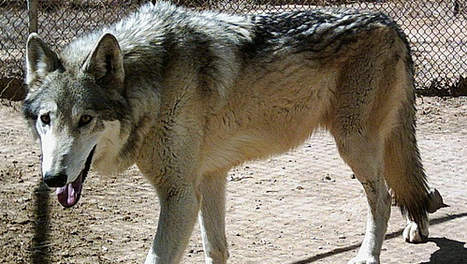
\includegraphics[width=0.9\textwidth]{WolfHond.jpg}
  \caption{Kruising tussen een wolf en een hond \cite{redactieHLN}}
  \label{fig:wolfhond}
\end{figure}
Als men denkt aan huisdieren denkt men natuurlijk aan de hond, de beste vriend van de mens. Daarom dat we even dieper in gaan op het leven van een hond na het verdwijnen van de mens. Zoals al eerder vermeld zullen kleine honden geen grote slaagkans op overleven hebben. Grote honden daarentegen hebben nog een groot deel van hun jachtinstinct kunnen behouden. Dit doordat deze honden vaak in de jacht gebruikt worden of dat er vaak actief mee gespeeld wordt. Deze honden hebben dan weer een grotere kans op overleven, zij zullen immers sneller gaan jagen om zo voedsel te vinden. Aangezien alle huisdieren in het begin nog in de stad zullen zijn, zullen de kleinere huisdieren er eerst aan moeten geloven. Wat ook wel interessant is, is het feit dat wilde dieren zoals wolven dichter naar de dorpen zullen komen. Dit brengt zich mee dat honden en wolven gaan kruisen en zo gaan zorgen voor nakomelingen. Dit zal er voor zorgen dat de hond na verloop van tijd zal verdwijnen en 'terug' zal evolueren naar de wolf, op figuur \ref{fig:wolfhond} is een foto te zien van een kruising tussen een wolf en een hond.
\subsection{Boerderijdieren}
De dieren op de boerderij leven altijd in gevangenschap, maar aangezien de elektriciteit na verloop van tijd zal uitvallen zullen veel van deze dieren uitbreken. Veel dieren zullen hierdoor prooi worden voor roofdieren of uitgebroken huisdieren. Andere dieren zullen vluchten en terug naar hun wilde vorm terugkeren. Denk zo maar aan wilde paarden.
\subsection{Dierentuin}
De dieren in de dierentuin zullen ook gevangen zitten in kooien en geen voedsel meer kunnen krijgen. Veel van deze dieren zullen kunnen uitbreken door hun instinct. Dit kan er voor zorgen dat er nijlpaarden door de rivieren in Zuid-Amerika zullen zwemmen of kamelen door de landschappen van Australi\"{e} zullen dwalen \cite{ASAPScience}.
\subsection{Wilde dieren}
Tenslotten gaan we het hebben over de dieren die in de wildernis leven. Deze dieren zijn op het eerste gezicht niet zo verwant met de mens maar niets is minder waar.
\newline
Zo zijn er dieren die schuw zijn van de mens en zich teruggetrokken hebben. Deze dieren zullen dichter tot de dorpen en steden komen doordat er geen mensen meer zijn waar ze bang voor moeten zijn. Dit zal er voor zorgen dat er terug wolven en grote katachtigen zullen verschijnen in onze landschappen.
\newline
De mens heeft er ook voor gezorgd dat veel dieren met uitsterven bedreigd zijn of al uitgestorven zijn. De dieren die momenteel met uitsterven bedreigd zijn zullen zich herstellen naar de normale proporties. Er is namelijk geen mens meer die leefruimte wegneemt of op ze jaagt. Zo zullen walvissen meer zeeruimte hebben en zich vermenigvuldigen naar de maximale capaciteit van onze oceanen \cite{LAPOutbreak}.

\newpage
\section{Constructies}
De mens heeft tal van constructies gebouwd tijdens zijn bestaan op de aarde. Denk zo aan de piramides in Egypte of het huis waar je nu in woont. Wat we zeker niet mogen vergeten zijn de ruimtetuigen die momenteel nog in een baan rond de aarde zitten. Maar wat gebeurt er met deze constructies nadat de mens verdwenen is? Er is namelijk niemand die de constructies zal repareren of renoveren. In dit hoofdstuk bekijken we gebouwen in de grote zin van het woord, we zullen het ook hebben over de ondergrondse tunnels voor de metro, monumenten...
\newline
\newline
Amper twee dagen na het verdwijnen van de mens zullen alle ondergrondse metrostations volgelopen zijn met water. Dit doordat het grondwater niet weggepompt zal worden. Een jaar hierna zullen alle ruimtetuigen neerstorten op de aarde doordat deze niet meer onder controle worden gehouden door mensen op aarde. Dit zal er uitzien als een gigantische sterrenregen. \cite{LAPOutbreak}
\newline
Na amper vijfentwintig jaar zal drie kwart van de bebouwde aarde terug begroeid zijn met vegetatie die daar behoort. Zo zullen onze steden veranderen in weilanden en bossen, terwijl steden zoals Las Vegas en Dubai zullen veranderen in woestijnen. De natuur neemt terug wat van hem is. \cite{ASAPScience, LAPOutbreak}
\newline
Onze huizen daarentegen zullen het langer volhouden, toch is dit een opvallend korte periode. Het zal namelijk vijftig tot honderd jaar duren voordat al onze huizen ingestort zullen zijn. We gaan er dan wel van uit dat er geen branden zijn ontstaan. Dit komt echter vaker voor zonder het toezicht van de mens. Wanneer namelijk \"{e}\"{e}n huis vuur vat, zal er niemand zijn om de vlammen onder controle te krijgen en het vuur zal zich dus onherroeppelijk verspreiden naar de omliggende constructies of natuur. Ook termieten zullen er voor zorgen dat vele huizen instorten. 
\newline
\begin{figure}
	\centering
	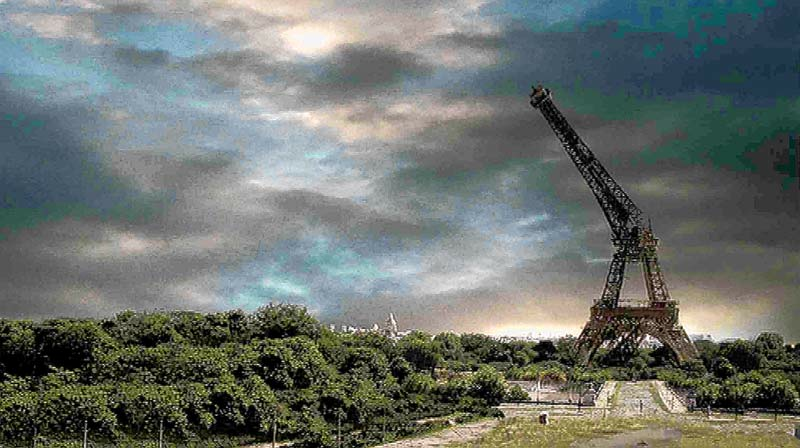
\includegraphics[width=0.9\textwidth]{EiffelToren.png}
	\caption{Instorten van de Eiffeltoren \cite{LAPOutbreak}}
	\label{fig:eiffel}
\end{figure}
\newline
Na ongeveer 300 jaar zullen de ijzeren constructies van de mens er ook aan moeten geloven. Zo zullen vele bruggen en ook de eiffeltoren (zoals te zien in figuur \ref{fig:eiffel}) er aan moeten geloven. Dit doordat het ijzer zal roesten. Corrosie zorgt er ook voor dat het ijzer uitzet. Dit zal er voor zorgen dat grote gebouwen, die veel ijzerwerk vereisen, zullen instorten. Na deze periode zal ook zo goed als elke dam ter wereld overstroomd of vernietigd zijn. Dit zal er voor zorgen dat Amerika bijvoorbeeld terug zal veranderen naar een moerassig landschap. Dit zorgt er dan weer voor dat vele dieren kunnen terugkeren naar hun oorspronkelijke woonplaats.
\newline
Na een ongeveer tienduizend jaar zullen er nog maar enkele overblijfselen van onze gebouwen te zien zijn, we hebben het dan bijvoorbeeld over de piramides of de Chinese Muur. \cite{LAPOutbreak}
\begin{thebibliography}{9}

\bibitem{redactieHLN}
  Redactie HLN,
  \emph{Vergeet uw trouwe hond, haal een halve wolf in huis},
  Het Laatste Nieuws,
  2009.
 \bibitem{ASAPScience}
  Asap Science,
  \emph{What if humans disappeared?},
  https://www.youtube.com/watch?v=guh7i7tHeZk,
  2015
 \bibitem{LAPOutbreak}
	Flight 33 Productions,
    \emph{Life After People},
    History,
    2008
\bibitem{WorldWithoutUs}
	Alan Weisman,
	\emph{The World Without Us},
	2007
\end{thebibliography}


\end{document}